%%%%%%%%%%%%%%%%%%%%%%%%%%%%%%%%%%%%%%%%%%%%%%%%%%%%%%%%%%%%%%%%%%%%%%%%%%%%%%%%%%%%%%%
%%%%%%%%%%%%%%%%%%%%%%%%%%%%%%%%%%%%%%%%%%%%%%%%%%%%%%%%%%%%%%%%%%%%%%%%%%%%%%%%%%%%%%%
%%%%%%%%%%%%%%%%%%%%%%%%%%%%%%%%%%%%%%%%%%%%%%%%%%%%%%%%%%%%%%%%%%%%%%%%%%%%%%%%%%%%%%%
\section{Regressão polinomial com
$h_{\VECTOR{c}}(x):~\mathbb{R} \rightarrow \mathbb{R}$}
\label{sec:theo:maphxr1r1}

\index{Problema inverso: Aplicado!Linear}
\index{Regressão não linear!Simples!Polinômio $h_{\VECTOR{c}}(x):~\mathbb{R} \rightarrow \mathbb{R}$}
\index{Regressão!Polinômio $h_{\VECTOR{c}}(x):~\mathbb{R} \rightarrow \mathbb{R}$}


\begin{theorem}[Regressão usando um polinômio 
$h_{\VECTOR{c}}(x)$ de grau $M$:]
\label{theo:maphxr1r1}
~\\
\begin{minipage}{0.4\textwidth}
\centering
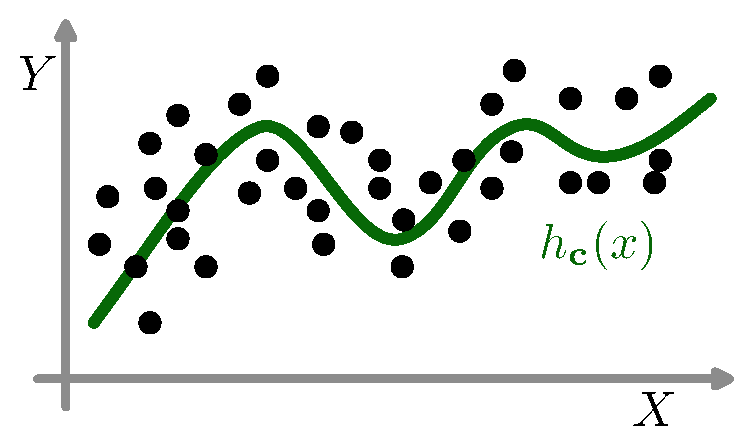
\includegraphics[width=0.95\linewidth]{chapters/mapeamento/mapeamento-hx.eps} 
\end{minipage}
\begin{minipage}{0.6\textwidth}
Dados
os escalares $x \in \mathbb{R}$, $y \in \mathbb{R}$ e $c_m \in \mathbb{R}$,
uma função polinomial $h_{\VECTOR{c}}:\mathbb{R} \rightarrow \mathbb{R}$, de grau $M$, e 
definida a Eq. (\ref{eq:maphxr1r1:1}),
\begin{equation}\label{eq:maphxr1r1:1}
y=h_{\VECTOR{c}}(x)\equiv \sum_{m=0}^{M}c_{m+1} x^m.
\end{equation}
Podemos afirmar que o vetor $\VECTOR{c}=[c_1~ c_2~ ...~ c_m~ ...~ c_{M+1}]^{\transpose}$ $\in \mathbb{R}^{M+1}$,
que minimiza o erro $e(\VECTOR{c})$,
\end{minipage}

\begin{equation}\label{eq:maphxr1r1:2}
%e(\VECTOR{c}) = ||h(\VECTOR{x})-\VECTOR{y}||_{\MATRIX{W}}^2 \equiv \sum_{n=1}^{N} w_n||h(x_n)-y_n||^2,
e(\VECTOR{c}) =  \sum_{n=1}^{N} w_n||h_{\VECTOR{c}}(x_n)-y_n||^2,
\end{equation}
proveniente de avaliar $N$ amostras $x_n$ e $y_n$ que não cumprem necessariamente a Eq. (\ref{eq:maphxr1r1:1}), 
representadas pelos vetores $\VECTOR{x}=[x_1~ x_2~ ...~ x_n~ ...~ x_N]^{\transpose}$ e 
$\VECTOR{y}=[y_1~ y_2~ ...~ y_n~ ...~ y_N]^{\transpose}$,
ponderados com os pesos $w_n \in \mathbb{R}_+$, 
representados pela matriz diagonal $\MATRIX{W}=\funcdiag([w_1~ w_2~ ...~ w_n~ ...~ w_N]^{\transpose})$;
pode ser achado\footnote{A demonstração pode ser vista na Prova \ref{proof:theo:maphxr1r1}.}, usando:
\begin{equation}\label{eq:maphxr1r1:3}
\VECTOR{c}=[\MATRIX{A}^{\transpose}\MATRIX{W}\MATRIX{A}]^{-1}\MATRIX{A}^{\transpose}\MATRIX{W}\VECTOR{y},
\end{equation}
sendo a matriz $\MATRIX{A}$ é definida como,
\begin{equation}\label{eq:maphxr1r1:4}
\MATRIX{A}\equiv \MATRIX{A}(\VECTOR{x})=\begin{bmatrix}
\VECTOR{a}_M(x_1)\\
\VECTOR{a}_M(x_2)\\
\vdots\\
\VECTOR{a}_M(x_N)\\
\end{bmatrix}, \qquad
\VECTOR{a}_M(x)=\begin{bmatrix}
1& x& x^2& \hdots & x^m& \hdots& x^M
\end{bmatrix}
\end{equation}

\end{theorem}


\begin{tcbattention}
\begin{itemize}
\item É importante lembrar que para que o vetor $\VECTOR{c}$
que minimiza $e(\VECTOR{c})$ tenha resposta única,
é necessário (porém não suficiente) que o número de amostras $N$ seja maior que a ordem $M$ do polinômio $h_{\VECTOR{c}}(x)$.

\item De forma exata, podemos afirmar que para que $\VECTOR{c}$ tenha resposta única,
deve existir inversa para a matriz $\MATRIX{A}^{\transpose}\MATRIX{W}\MATRIX{A}$.

\end{itemize}
\end{tcbattention}


%%%%%%%%%%%%%%%%%%%%%%%%%%%%%%%%%%%%%%%%%%%%%%%%%%%%%%%%%%%%%%%%%%%%%%%%%%%%%%%%
\subsection{Exemplos de regressão com um polinômio
$h_{\VECTOR{c}}(x):~\mathbb{R} \rightarrow \mathbb{R}$ de grau $M$ }

\begin{example}\label{ex:theo:maphxr1r1}
Conhecida as $N=16$ amostras $x_n$ e $y_n$, 
mostradas nas  Tabelas \ref{table:theo:maphxr1r1:xn} e \ref{table:theo:maphxr1r1:yn},
achar o polinômio $h_{\VECTOR{c}}(x)$ de grau $M=2$, 
que gere o menor erro $e(\VECTOR{c}) =  \sum_{n=1}^{N} ||h_{\VECTOR{c}}(x_n)-y_n||^2$.
\end{example}


\begin{table}[h!]
\centering
\begin{tabular}{|c|c|c|c|c|c|c|c|c|} 
 \hline
$n$   & 1 & 2 & 3 & 4 & 5 & 6 & 7 & 8\\ \hline
$x_n$ & 0.10461 & 0.29614 & 1.63968 & 1.89586 & 3.17301 & 3.68811 & 3.75758 & 3.96560 \\ \hline
 \hline
$n$   & 9 & 10 & 11 & 12 & 13 & 14 & 15 & 16\\  \hline
$x_n$ & 6.09526 & 6.12999 & 6.81288 & 8.33457 & 8.74851 & 8.81418 & 9.16269 & 9.30314 \\ \hline
\end{tabular}
\caption{Valores $x_n$.}
\label{table:theo:maphxr1r1:xn}
\end{table}

\begin{table}[h!]
\centering
\begin{tabular}{|c|c|c|c|c|c|c|c|c|} 
 \hline
$n$   & 1 & 2 & 3 & 4 & 5 & 6 & 7 & 8\\ \hline
$y_n$ & -1.3158 & 1.6375 & 2.9296 & 2.3120 & 12.6019 & 16.1430 & 11.4531 & 15.7617  \\ \hline
 \hline
$n$   & 9 & 10 & 11 & 12 & 13 & 14 & 15 & 16\\  \hline
$y_n$ & 34.2272 & 39.0406 & 46.3776 & 67.6390 & 79.6249 & 76.2655 & 84.2627 & 89.3032 \\ \hline
\end{tabular}
\caption{Valores $y_n$.}
\label{table:theo:maphxr1r1:yn}
\end{table}

\begin{SolutionT}[Relativa ao Exemplo \ref{ex:theo:maphxr1r1}:]\label{sol:theo:maphxr1r1}
Para obter o polinômio $h_{\VECTOR{c}}(x)$ de grau $M=2$, 
que gere o menor erro $e(\VECTOR{c}) =  \sum_{n=1}^{N} ||h_{\VECTOR{c}}(x_n)-y_n||^2$,
usamos a Eq. (\ref{eq:maphxr1r1:1}), 
onde o vetor $\VECTOR{c}$ é calculado usando a Eq. (\ref{eq:maphxr1r1:3}),
na qual obtemos que $\VECTOR{c}=[0.35232\quad -0.24794\quad 1.03077]^{\transpose}$, de modo que
\begin{equation}
\begin{matrix}
h_{\VECTOR{c}}(x) & = & c_1+c_2 x+c_3 x^2 \\
                ~ & = & 0.35232 -0.24794 x + 1.03077 x^2
\end{matrix}
\end{equation}
    \begin{figure}[!h]
        \centering
        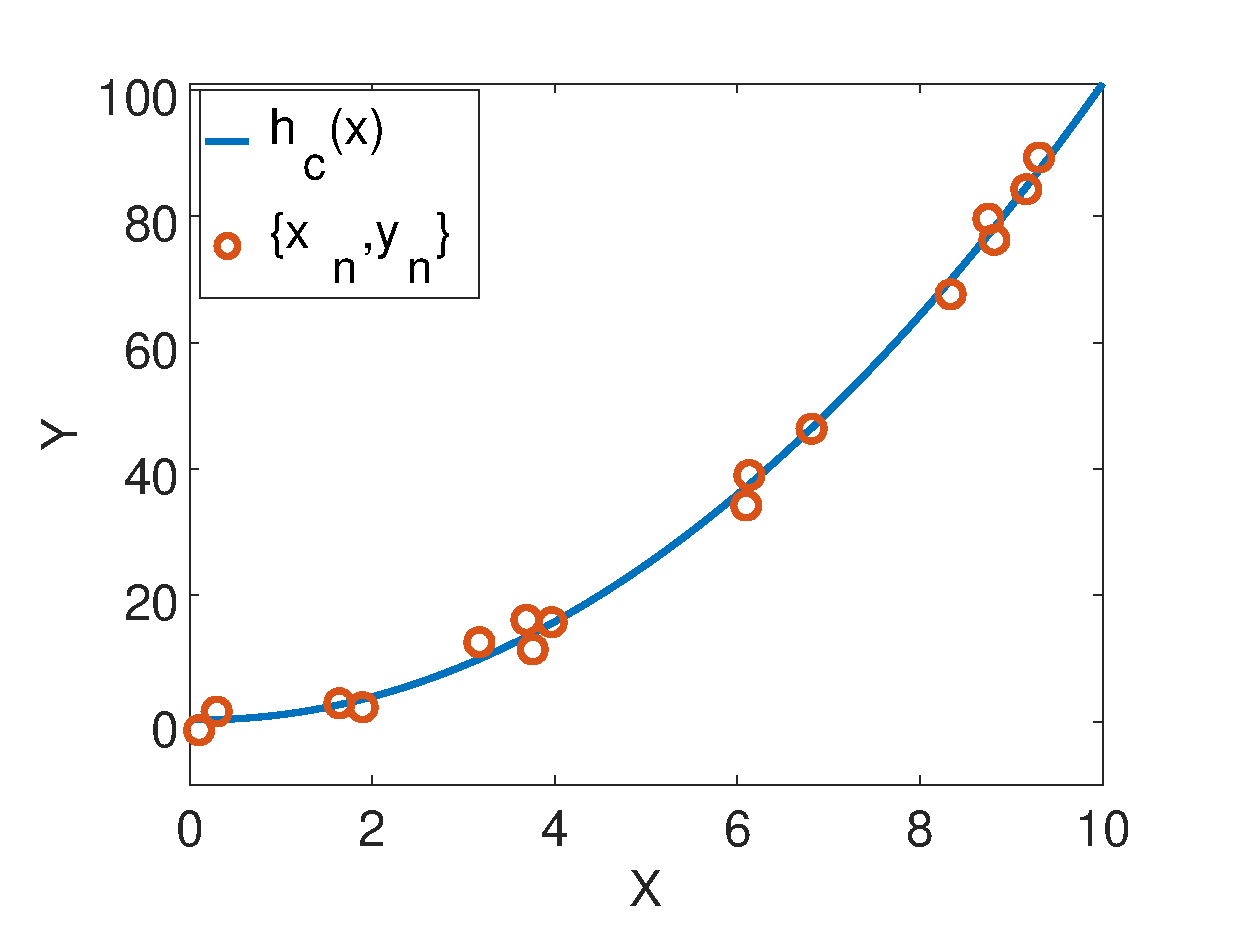
\includegraphics[width=0.49\textwidth]{chapters/mapeamento/mfiles/mapeamentor1r1/minimizando_hx.eps}
        \caption{Gráfico das amostras $\{x_n,y_n\}$ e da curva $x$ vs. $h_{\VECTOR{c}}(x)$.}
        \label{fig:theo:maphxr1r1:xnyn}
    \end{figure}

\end{SolutionT}


